% =============================================================================
% Figure 1, panel (C) — proliferation drives cellular extrusion
%   Left  : a cell in the monolayer divides parallel to the membrane; the two
%           daughters (solid) fill the footprint of the parent (dotted).
%   Right : as the daughters grow the row can no longer hold them and one cell
%           is pushed off the membrane into the lumen, starting a second layer.
% Standalone:  pdflatex fig_extrusion.tex
% =============================================================================
\documentclass[tikz,border=6pt]{standalone}
\usepackage{amsmath}
\usetikzlibrary{arrows.meta,calc}

\definecolor{BMcol}{RGB}{40,40,40}
\definecolor{EPcol}{RGB}{70,120,180}

\begin{document}
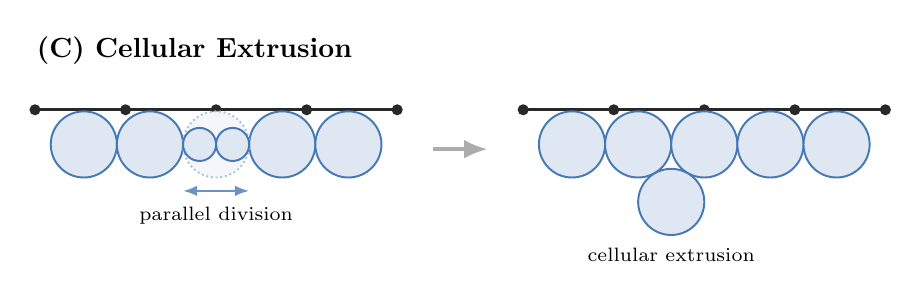
\begin{tikzpicture}[
  >=Latex,
  ep/.style={circle,draw=EPcol,fill=EPcol!18,line width=.7pt,minimum size=0.84cm},
  daughter/.style={circle,draw=EPcol,fill=EPcol!18,line width=.7pt,minimum size=0.42cm},
  parent/.style={circle,draw=EPcol!45,densely dotted,fill=EPcol!6,
                 line width=.7pt,minimum size=0.84cm},
  bmnode/.style={circle,fill=BMcol,inner sep=0pt,minimum size=4pt},
  sml/.style={font=\scriptsize},
]

\node[font=\bfseries,anchor=west] at (-2.40,2.30)
     {(C) Cellular Extrusion};

% ------------------------------- membrane (both stages) ---------------------
\foreach \dx in {0,6.2}{
  \begin{scope}[shift={(\dx,0)}]
    \draw[BMcol,line width=1.2pt] (-2.3,1.55) -- (2.3,1.55);
    \foreach \x in {-2.3,-1.15,0,1.15,2.3}{\node[bmnode] at (\x,1.55) {};}
  \end{scope}
}

% ================================ before: division ==========================
\begin{scope}
  \foreach \x in {-1.68,-0.84,0.84,1.68}{\node[ep] at (\x,1.11) {};}

  \node[parent]   at (0,1.11) {};
  \node[daughter] at (-0.21,1.11) {};
  \node[daughter] at ( 0.21,1.11) {};

  \draw[EPcol!80,{Latex[length=1.8mm]}-{Latex[length=1.8mm]},line width=.8pt]
        (-0.42,0.52) -- (0.42,0.52);
  \node[sml,anchor=north] at (0,0.44) {parallel division};
\end{scope}

% ---------------------------------- then --------------------------------
\draw[gray!65,line width=1.4pt,-{Latex[length=3mm,width=2.4mm]}] (2.75,1.05) -- (3.45,1.05);

% ================================ after: extrusion ==========================
\begin{scope}[shift={(6.2,0)}]
  \foreach \x in {-1.68,-0.84,0,0.84,1.68}{\node[ep] at (\x,1.11) {};}

  % extruded cell nestled in the gap between two neighbours (touching both)
  \node[ep] at (-0.42,0.38) {};
  \node[sml,anchor=north] at (-0.42,-0.08) {cellular extrusion};
\end{scope}

\end{tikzpicture}
\end{document}
